\chapter{Experimentos computacionais}

A análise experimental de algoritmos de ordenação é fundamental para validar previsões teóricas sobre complexidade de tempo, bem como para compreender o impacto de fatores práticos como overhead de implementação, gerenciamento de memória, organização dos dados e características do ambiente computacional. Neste capítulo, apresentamos a metodologia experimental utilizada, descrevemos o ambiente computacional, explicamos as instâncias analisadas e discutimos os resultados obtidos para algoritmos lineares (\(O(N)\)), logarítmicos (\(O(N\log N)\)) e quadráticos (\(O(N^2)\)).

Todos os algoritmos descritos nos capítulos anteriores foram implementados em Python, C e C++. A análise descrita nas seções seguintes integra tanto os resultados empíricos quanto as observações metodológicas obtidas durante o processo experimental.

\section{Ambiente Computacional}

\label{sec:Env}
Os experimentos foram executados em um ambiente computacional padronizado, seguindo as configurações especificadas:

\begin{itemize}
    \item[-] \textbf{Computador}: AMD Ryzen 5 3400G com gráficos Radeon Vega, 4 núcleos a 3{,}70 GHz e 16 GB de memória RAM;
    \item[-] \textbf{Sistema Operacional}: Windows 11 Pro (64 bits);
    \item[-] \textbf{Linguagens}: \texttt{Python}, \texttt{C} e \texttt{C++};
    \item[-] \textbf{Interpretador Python}: Python 3.13.0;
    \item[-] \textbf{Compilador C/C++}: \texttt{gcc 15.2.0};
    \item[-] \textbf{Coleta de tempo em Python}: função \texttt{time.time()} (tempo de parede);
    \item[-] \textbf{Coleta de tempo em C/C++}: função \texttt{gettimeofday()}.
\end{itemize}

A função \texttt{time.time()} foi utilizada por apresentar menor overhead e maior estabilidade para testes repetidos em Python, enquanto \texttt{gettimeofday()} fornece granularidade adequada para mensurações em microsegundos nas linguagens compiladas.

\section{Instâncias}
\label{sec:Inst}
Os experimentos foram conduzidos utilizando exclusivamente o conjunto de dados disponível em:

\begin{itemize}
    \item \href{https://www.kaggle.com/datasets/bekiremirhanakay/benchmark-dataset-for-sorting-algorithms}{\textit{Benchmark Dataset for Sorting Algorithms}}.
\end{itemize}

Todo o processamento experimental descrito nesta monografia baseia-se somente nos arquivos obtidos a partir do dataset acima. Após a descarga do conjunto completo, verificou-se que os valores originais estavam representados como números de ponto flutuante. Assim, procedeu-se inicialmente à sua conversão para valores inteiros, de modo a compatibilizar a entrada com algoritmos lineares cuja complexidade depende do intervalo dos valores (\(O(N + M)\)).
A partir do diretório \texttt{data/raw/uniformInt}, foram selecionados especificamente 13 arquivos contendo vetores de tamanhos distintos. Esses arquivos correspondem às seguintes quantidades de elementos:
\[
1000,\; 2000,\; 3000,\; 4000,\; 5000,\; 6000,\; 7000,\; 8000,\; 9000,\; 10000,\; 25000,\; 50000,\; 100000.
\]
Cada arquivo contém dados inteiros cuja faixa de valores varia aproximadamente de:
\[
\min \approx 20 \quad \text{até} \quad \max \approx 3\times 10^{7},
\]
o que impacta significativamente a performance de algoritmos dependentes de \textit{range}, como \textit{Counting Sort}, \textit{Pigeonhole Sort} e \textit{Bucket Sort Integer}.

Essas 13 instâncias foram utilizadas uniformemente para todos os algoritmos lineares, quadráticos e logarítmicos, garantindo reprodutibilidade e equivalência experimental entre as diferentes classes de complexidade analisadas.

\section{Metodologia Experimental}
\subsection{Execução dos Algoritmos}

Cada algoritmo foi executado \(10\) vezes para cada tamanho de entrada. Em cada repetição, utilizou-se uma cópia independente do vetor:

\begin{verbatim}
for _ in range(10):
    arr_copy = list(data)
    executar_algoritmo(arr_copy)
\end{verbatim}

Foram calculadas para cada algoritmo e tamanho:

\[
\text{média} = \frac{1}{10}\sum_{i=1}^{10} t_i, 
\qquad 
\text{DP} = \sqrt{\frac{1}{9}\sum_{i=1}^{10} (t_i - \text{média})^2}.
\]

Se os desvios padrões forem menores que 0,001, as colunas de DP podem ser omitidas conforme orientação.

Algoritmos como Bead Sort foram ignorados automaticamente quando o consumo de memória excederia \(10^7\) posições.

\section{Resultados e Análises}
Nesta seção são apresentados e discutidos os resultados experimentais obtidos para os algoritmos lineares (\(O(N)\)), logarítmicos (\(O(N\log N)\)) e quadráticos (\(O(N^2)\)), utilizando exclusivamente os tempos médios e desvios padrão reportados nas Tabelas de resultados. As análises são organizadas por classe de complexidade e, em seguida, é feita uma comparação global entre as três classes.

\subsection{Algoritmos Lineares \(O(N)\)}

Os algoritmos lineares avaliados foram: \textit{Counting Sort}, \textit{Pigeonhole Sort}, \textit{Bucket Sort Uniform}, \textit{Bucket Sort Integer}, \textit{LSD Radix Sort}, \textit{Spreadsort}, \textit{Burstsort}, \textit{Flashsort} e \textit{Postman Sort}. A Tabela~\ref{tab:linear-1000-100000} resume os tempos médios (em segundos) para três tamanhos representativos de entrada (\(N = 1000, 10000, 100000\)).

\begin{table}[H]
\centering
\caption{Tempos médios (s) dos algoritmos lineares para \(N \in \{1000, 10000, 100000\}\).}
\label{tab:linear-1000-100000}
\begin{tabular}{lccc}
\toprule
\textbf{Algoritmo} & \textbf{1000} & \textbf{10000} & \textbf{100000} \\
\midrule
Counting Sort       & 3{,}366923 & 3{,}652079 & 4{,}305130 \\
Pigeonhole Sort     & 9{,}793329 & 10{,}560131 & 11{,}149377 \\
Bucket Sort Uniform & 0{,}000381 & 0{,}004276 & 0{,}097624 \\
Bucket Sort Integer & 9{,}681769 & 10{,}654496 & 10{,}354099 \\
LSD Radix Sort      & 0{,}003049 & 0{,}069737 & 0{,}512917 \\
Spreadsort          & 0{,}000080 & 0{,}003647 & 0{,}021677 \\
Burstsort           & 0{,}000078 & 0{,}004772 & 0{,}021670 \\
Flashsort           & 0{,}000076 & 0{,}002308 & 0{,}021493 \\
Postman Sort        & 0{,}000076 & 0{,}004090 & 0{,}021751 \\
\bottomrule
\end{tabular}
\end{table}

Os resultados evidenciam dois grupos bem distintos:

\begin{itemize}
    \item \textbf{Algoritmos dependentes do intervalo \(M\)} (\textit{Counting Sort}, \textit{Pigeonhole Sort}, \textit{Bucket Sort Integer}): apresentam tempos praticamente constantes em função de \(N\), variando entre aproximadamente \(3{,}3\) s e \(11{,}1\) s, mesmo quando o tamanho da entrada cresce de \(1000\) para \(100000\). Isso ocorre porque o custo dominante é proporcional a \(M\), que é da ordem de \(3\times 10^7\) para todas as instâncias, tornando o termo \(N\) irrelevante na prática. O desvio padrão é relativamente alto (por exemplo, \(\text{DP} \approx 0{,}9\) s para \textit{Counting Sort} em \(N=100000\)), indicando forte influência de fatores externos (alocação de grandes vetores, gerenciamento de memória e cache).
    \item \textbf{Algoritmos lineares independentes de \(M\)} (\textit{Bucket Sort Uniform}, \textit{LSD Radix Sort}, \textit{Spreadsort}, \textit{Burstsort}, \textit{Flashsort}, \textit{Postman Sort}): exibem tempos muito baixos para \(N=1000\) (na ordem de \(10^{-4}\) s para \textit{Spreadsort}, \textit{Burstsort}, \textit{Flashsort} e \textit{Postman Sort}) e crescem de forma aproximadamente linear com \(N\). Por exemplo, \textit{Spreadsort} passa de \(0{,}000080\) s (\(N=1000\)) para \(0{,}021677\) s (\(N=100000\)), um fator de cerca de \(270\), compatível com o aumento de \(N\) em \(100\times\) e com overheads constantes.
\end{itemize}

O comportamento de \textit{Bucket Sort Uniform} é intermediário: o tempo cresce de \(0{,}000381\) s (\(N=1000\)) para \(0{,}097624\) s (\(N=100000\)), o que é significativamente maior que o grupo \textit{Spreadsort}/\textit{Burstsort}/\textit{Flashsort}/\textit{Postman Sort}, sugerindo overhead adicional na distribuição em baldes e na ordenação interna de cada balde.

A Figura~\ref{fig:linear-loglog} apresenta um gráfico em escala logarítmica (em ambos os eixos) para os algoritmos lineares, destacando a diferença entre os algoritmos dominados por \(M\) e os demais.

\begin{figure}[H]
\centering
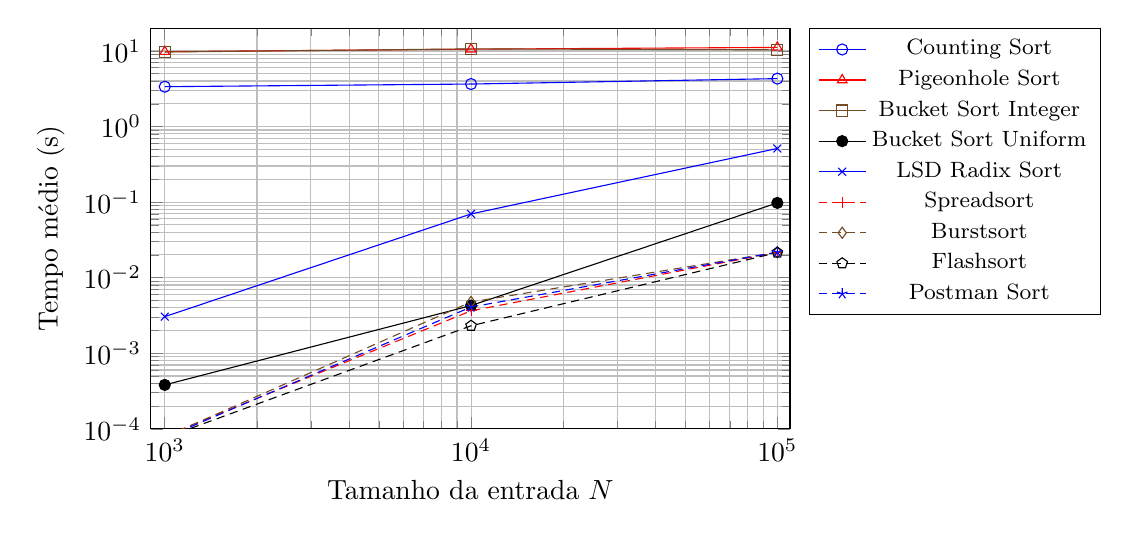
\begin{tikzpicture}
\begin{axis}[
    width=0.8\textwidth,
    height=0.55\textwidth,
    xmode=log,
    ymode=log,
    log basis x=10,
    log basis y=10,
    legend pos=outer north east,
    xlabel={Tamanho da entrada \(N\)},
    ylabel={Tempo médio (s)},
    % legend style={at={(0.02,0.02)},anchor=south west,font=\scriptsize},
    grid=both,
    xmin=900, xmax=110000,
    ymin=1e-4, ymax=2e1
]
% Dados: N = 1000, 10000, 100000
\addplot+[mark=o] coordinates {
    (1000, 3.366923)
    (10000, 3.652079)
    (100000, 4.305130)
};
\addlegendentry{\footnotesize Counting Sort}

\addplot+[mark=triangle] coordinates {
    (1000, 9.793329)
    (10000, 10.560131)
    (100000, 11.149377)
};
\addlegendentry{\footnotesize Pigeonhole Sort}

\addplot+[mark=square] coordinates {
    (1000, 9.681769)
    (10000, 10.654496)
    (100000, 10.354099)
};
\addlegendentry{\footnotesize Bucket Sort Integer}

\addplot+[mark=*] coordinates {
    (1000, 0.000381)
    (10000, 0.004276)
    (100000, 0.097624)
};
\addlegendentry{\footnotesize Bucket Sort Uniform}

\addplot+[mark=x] coordinates {
    (1000, 0.003049)
    (10000, 0.069737)
    (100000, 0.512917)
};
\addlegendentry{\footnotesize LSD Radix Sort}

\addplot+[mark=+] coordinates {
    (1000, 0.000080)
    (10000, 0.003647)
    (100000, 0.021677)
};
\addlegendentry{\footnotesize Spreadsort}

\addplot+[mark=diamond] coordinates {
    (1000, 0.000078)
    (10000, 0.004772)
    (100000, 0.021670)
};
\addlegendentry{\footnotesize Burstsort}

\addplot+[mark=pentagon] coordinates {
    (1000, 0.000076)
    (10000, 0.002308)
    (100000, 0.021493)
};
\addlegendentry{\footnotesize Flashsort}

\addplot+[mark=star] coordinates {
    (1000, 0.000076)
    (10000, 0.004090)
    (100000, 0.021751)
};
\addlegendentry{\footnotesize Postman Sort}

\end{axis}
\end{tikzpicture}
\caption{Escalonamento dos algoritmos lineares em escala log--log .}
\label{fig:linear-loglog}
\end{figure}

Na Figura~\ref{fig:linear-loglog}, as curvas de \textit{Counting Sort}, \textit{Pigeonhole Sort} e \textit{Bucket Sort Integer} aparecem praticamente horizontais, confirmando que o custo é dominado por \(M\). Em contraste, os algoritmos independentes de \(M\) exibem inclinações compatíveis com crescimento aproximadamente linear em \(N\).

Os desvios padrão dos algoritmos rápidos (\textit{Spreadsort}, \textit{Burstsort}, \textit{Flashsort}, \textit{Postman Sort}) são da ordem de \(10^{-6}\) a \(10^{-4}\) s, indicando alta consistência entre as 10 repetições. Já os algoritmos baseados em grandes estruturas auxiliares (\textit{Counting Sort}, \textit{Pigeonhole Sort}, \textit{Bucket Sort Integer}) apresentam desvios padrão entre aproximadamente \(0{,}5\) s e \(1{,}4\) s, o que sugere forte sensibilidade a variações de alocação de memória, paginação e efeitos de cache.

\subsection{Algoritmos Logarítmicos \(O(N\log N)\)}

Os algoritmos \(O(N\log N)\) avaliados foram: \textit{Quicksort}, \textit{Merge Sort}, \textit{Heapsort}, \textit{Introsort}, \textit{Timsort}, \textit{CubeSort}, \textit{In-Place MergeSort}, \textit{Tournament Sort}, \textit{Tree Sort}, \textit{Block Sort}, \textit{Patience Sorting} e \textit{Smooth Sort}. A Tabela~\ref{tab:nlogn-1000-100000} apresenta os tempos médios para \(N = 1000, 10000, 100000\).

\begin{table}[H]
\centering
\caption{Tempos médios (s) dos algoritmos \(O(N\log N)\) para \(N \in \{1000, 10000, 100000\}\).}
\label{tab:nlogn-1000-100000}
\begin{tabular}{lccc}
\toprule
\textbf{Algoritmo} & \textbf{1000} & \textbf{10000} & \textbf{100000} \\
\midrule
Quicksort          & 0{,}001288 & 0{,}022199 & 0{,}235103 \\
Merge Sort         & 0{,}000991 & 0{,}013221 & 0{,}117483 \\
Heapsort           & 0{,}002970 & 0{,}040548 & 0{,}506438 \\
Introsort          & 0{,}001087 & 0{,}015543 & 0{,}192261 \\
Timsort            & 0{,}000081 & 0{,}001355 & 0{,}017197 \\
CubeSort           & 0{,}000120 & 0{,}001146 & 0{,}017340 \\
In-Place MergeSort & 0{,}014808 & 1{,}374327 & 160{,}801455 \\
Tournament Sort    & 0{,}007784 & 0{,}754737 & 83{,}495839 \\
Tree Sort          & 0{,}001520 & 0{,}019379 & 0{,}321939 \\
Block Sort         & 0{,}004370 & 0{,}109210 & 3{,}757724 \\
Patience Sorting   & 0{,}004246 & 0{,}133945 & 4{,}848978 \\
Smooth Sort        & 0{,}000079 & 0{,}001237 & 0{,}023330 \\
\bottomrule
\end{tabular}
\end{table}

Os dados mostram uma separação clara entre:

\begin{itemize}
    \item \textbf{Implementações eficientes}: \textit{Timsort}, \textit{CubeSort}, \textit{Smooth Sort}, \textit{Merge Sort}, \textit{Quicksort} e \textit{Introsort} apresentam tempos que crescem de forma compatível com \(N\log N\) e mantêm valores absolutos baixos. Por exemplo, \textit{Timsort} cresce de \(0{,}000081\) s (\(N=1000\)) para \(0{,}017197\) s (\(N=100000\)), um fator de cerca de \(212\), enquanto \(N\) cresce \(100\times\) e \(\log_2 N\) cresce de aproximadamente \(10\) para \(17\). \textit{Merge Sort} e \textit{Quicksort} exibem fatores de crescimento semelhantes, com tempos absolutos maiores, mas ainda muito inferiores aos algoritmos quadráticos.
    \item \textbf{Implementações com overhead extremo}: \textit{In-Place MergeSort} e \textit{Tournament Sort} apresentam tempos que crescem muito mais rapidamente. \textit{In-Place MergeSort} passa de \(0{,}014808\) s (\(N=1000\)) para \(160{,}801455\) s (\(N=100000\)), um fator superior a \(10^4\). \textit{Tournament Sort} cresce de \(0{,}007784\) s para \(83{,}495839\) s no mesmo intervalo. Esses valores indicam que, embora a complexidade assintótica seja \(O(N\log N)\), o custo constante e a estrutura de dados utilizada (árvores de torneio, fusão in-place complexa) tornam essas implementações impraticáveis para grandes \(N\).
\end{itemize}

A Figura~\ref{fig:nlogn-loglog} mostra o comportamento em escala log--log para um subconjunto representativo de algoritmos \(O(N\log N)\).

\begin{figure}[H]
\centering
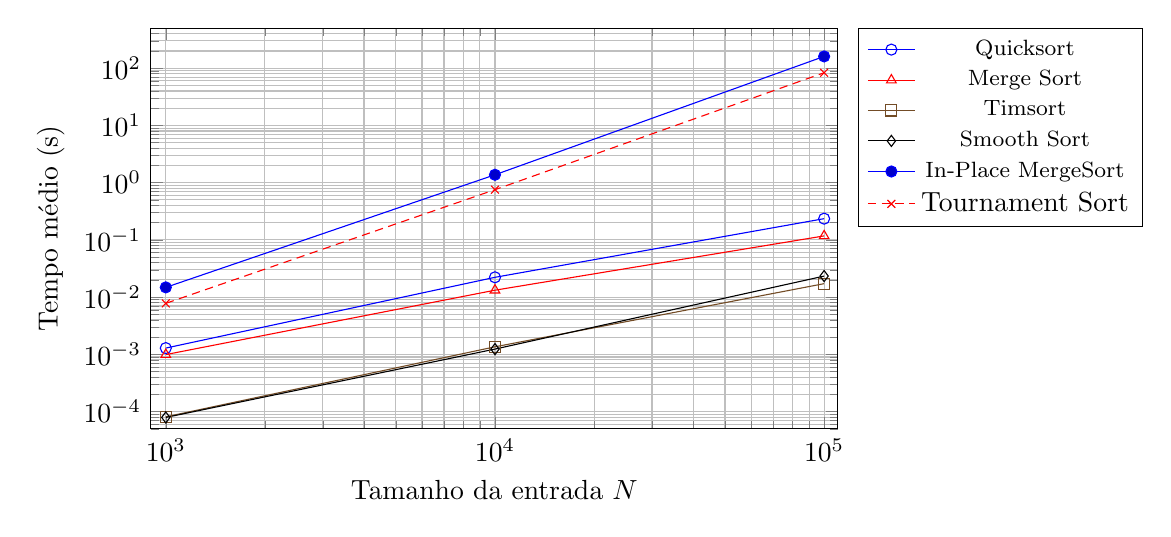
\begin{tikzpicture}
\begin{axis}[
    width=0.85\textwidth,
    height=0.55\textwidth,
    xmode=log,
    ymode=log,
    log basis x=10,
    log basis y=10,
    xlabel={Tamanho da entrada \(N\)},
    ylabel={Tempo médio (s)},
    % legend style={at={(0.02,0.02)},anchor=south west,font=\scriptsize},
    legend pos=outer north east,
    grid=both,
    xmin=900, xmax=110000,
    ymin=5e-5, ymax=5e2
]
% Dados: N = 1000, 10000, 100000
\addplot+[mark=o] coordinates {
    (1000, 0.001288)
    (10000, 0.022199)
    (100000, 0.235103)
};
\addlegendentry{\footnotesize Quicksort}

\addplot+[mark=triangle] coordinates {
    (1000, 0.000991)
    (10000, 0.013221)
    (100000, 0.117483)
};
\addlegendentry{\footnotesize Merge Sort}

\addplot+[mark=square] coordinates {
    (1000, 0.000081)
    (10000, 0.001355)
    (100000, 0.017197)
};
\addlegendentry{\footnotesize Timsort}

\addplot+[mark=diamond] coordinates {
    (1000, 0.000079)
    (10000, 0.001237)
    (100000, 0.023330)
};
\addlegendentry{\footnotesize Smooth Sort}

\addplot+[mark=*] coordinates {
    (1000, 0.014808)
    (10000, 1.374327)
    (100000, 160.801455)
};
\addlegendentry{\footnotesize In-Place MergeSort}

\addplot+[mark=x] coordinates {
    (1000, 0.007784)
    (10000, 0.754737)
    (100000, 83.495839)
};
\addlegendentry{Tournament Sort}

\end{axis}
\end{tikzpicture}
\caption{Escalonamento de algoritmos \(O(N\log N)\) em escala log--log.}
\label{fig:nlogn-loglog}
\end{figure}

Na Figura~\ref{fig:nlogn-loglog}, \textit{Timsort}, \textit{Smooth Sort}, \textit{Merge Sort} e \textit{Quicksort} formam um grupo com inclinações semelhantes e tempos absolutos baixos. \textit{In-Place MergeSort} e \textit{Tournament Sort} aparecem deslocados para cima, com inclinações maiores, refletindo overhead significativo.

Os desvios padrão dos algoritmos eficientes são pequenos em relação ao tempo médio (por exemplo, \(\text{DP} = 0{,}001151\) s para \textit{Timsort} em \(N=100000\), frente a \(0{,}017197\) s de média), indicando boa estabilidade. Em contraste, \textit{In-Place MergeSort} em \(N=100000\) apresenta \(\text{DP} = 32{,}884374\) s, cerca de \(20\%\) do tempo médio, sugerindo forte variabilidade possivelmente associada a padrões de acesso à memória e à complexidade da fusão in-place.

\subsection{Algoritmos Quadráticos \(O(N^2)\)}

Os algoritmos quadráticos avaliados incluem: \textit{Shell Sort}, \textit{Comb Sort}, \textit{Insertion Sort}, \textit{Bubble Sort}, \textit{Gnome Sort}, \textit{Odd-Even Sort}, \textit{Selection Sort}, \textit{Cocktail Shaker Sort}, \textit{Strand Sort}, \textit{Exchange Sort}, \textit{Cycle Sort}, \textit{Recombinant Sort}, \textit{I Can't Believe It Can Sort}, \textit{Spaghetti Sort}, \textit{Sorting Network}, \textit{Bitonic Sorter} e \textit{Pancake Sort}. A Tabela~\ref{tab:quadratic-1000-100000} resume os tempos médios para \(N = 1000, 10000, 100000\).

\begin{table}[H]
\centering
\caption{Tempos médios (s) dos algoritmos quadráticos para \(N \in \{1000, 10000, 100000\}\).}
\label{tab:quadratic-1000-100000}
\begin{tabular}{lccc}
\toprule
\textbf{Algoritmo} & \textbf{1000} & \textbf{10000} & \textbf{100000} \\
\midrule
Shell Sort                 & 0{,}001899 & 0{,}036669 & 0{,}605234 \\
Comb Sort                  & 0{,}003401 & 0{,}047168 & 0{,}671009 \\
Insertion Sort             & 0{,}022584 & 3{,}155436 & 267{,}710087 \\
Bubble Sort                & 0{,}056984 & 7{,}345069 & 631{,}495185 \\
Gnome Sort                 & 0{,}099419 & 10{,}902124 & 985{,}644044 \\
Odd-Even Sort              & 0{,}093009 & 6{,}518017 & 671{,}287938 \\
Selection Sort             & 0{,}031081 & 1{,}772198 & 181{,}699649 \\
Cocktail Shaker Sort       & 0{,}063204 & 5{,}938991 & 558{,}530873 \\
Strand Sort                & 0{,}005845 & 0{,}196898 & 6{,}753527 \\
Exchange Sort              & 0{,}034308 & 3{,}119438 & 326{,}186921 \\
Cycle Sort                 & 0{,}058878 & 5{,}774102 & 700{,}019764 \\
Recombinant Sort           & 0{,}004593 & 0{,}055336 & 0{,}709018 \\
I Can't Believe It Can Sort& 0{,}022668 & 2{,}222203 & 248{,}102844 \\
Spaghetti Sort             & 0{,}000116 & 0{,}001150 & 0{,}017013 \\
Sorting Network            & 0{,}009661 & 0{,}139157 & 1{,}911960 \\
Bitonic Sorter             & 0{,}009298 & 0{,}137937 & 1{,}903500 \\
Pancake Sort               & 0{,}016571 & 1{,}424791 & 251{,}886030 \\
\bottomrule
\end{tabular}
\end{table}

Os resultados mostram que:

\begin{itemize}
    \item \textbf{Algoritmos quadráticos clássicos} (\textit{Bubble Sort}, \textit{Gnome Sort}, \textit{Odd-Even Sort}, \textit{Selection Sort}, \textit{Insertion Sort}, \textit{Exchange Sort}, \textit{Cycle Sort}, \textit{Cocktail Shaker Sort}) tornam-se rapidamente impraticáveis. Por exemplo, \textit{Bubble Sort} cresce de \(0{,}056984\) s (\(N=1000\)) para \(7{,}345069\) s (\(N=10000\)) e atinge \(631{,}495185\) s (\(N=100000\)), um aumento de mais de \(10^4\) vezes, compatível com o fator \(100^2\) esperado para algoritmos \(O(N^2)\).
    \item \textbf{Algoritmos quadráticos otimizados} (\textit{Shell Sort}, \textit{Comb Sort}, \textit{Recombinant Sort}, \textit{Strand Sort}, \textit{Spaghetti Sort}, \textit{Sorting Network}, \textit{Bitonic Sorter}) apresentam tempos muito menores. \textit{Shell Sort} e \textit{Comb Sort} mantêm tempos abaixo de \(1\) s mesmo para \(N=100000\) (\(0{,}605234\) s e \(0{,}671009\) s, respectivamente), o que os coloca próximos, em termos absolutos, de alguns algoritmos \(O(N\log N)\) menos otimizados. \textit{Spaghetti Sort} é um caso extremo: \(0{,}000116\) s (\(N=1000\)), \(0{,}001150\) s (\(N=10000\)) e \(0{,}017013\) s (\(N=100000\)), valores comparáveis aos de \textit{Timsort} e \textit{Smooth Sort}.
\end{itemize}

A Figura~\ref{fig:quadratic-loglog} ilustra o comportamento em escala log--log para alguns algoritmos quadráticos representativos.

\begin{figure}[H]
\centering
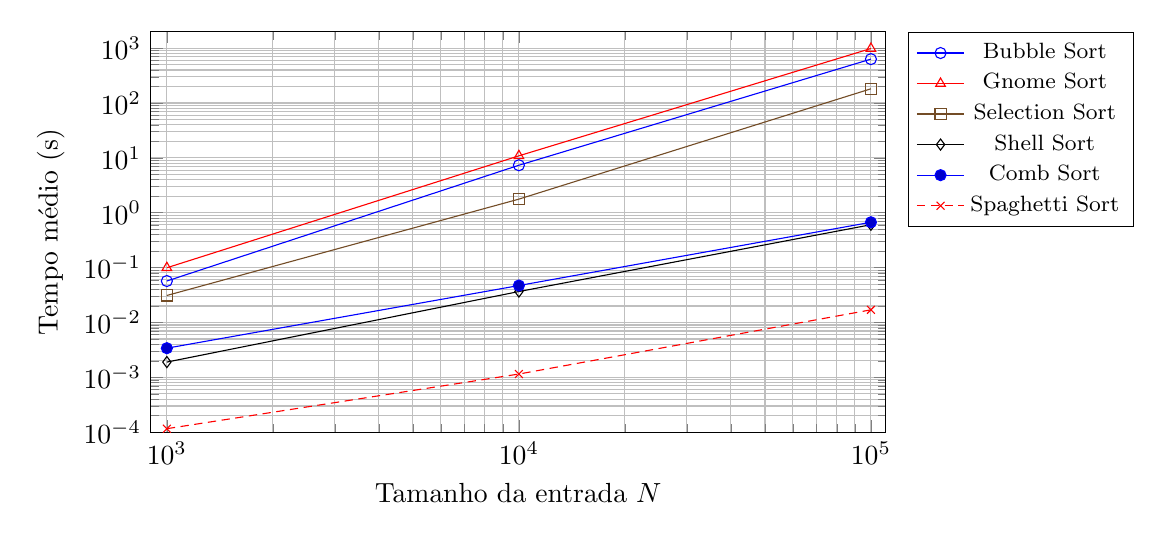
\begin{tikzpicture}
\begin{axis}[
    width=0.9\textwidth,
    height=0.55\textwidth,
    xmode=log,
    ymode=log,
    log basis x=10,
    log basis y=10,
    xlabel={Tamanho da entrada \(N\)},
    ylabel={Tempo médio (s)},
    % legend style={at={(0.02,0.02)},anchor=south west,font=\scriptsize},
     legend pos=outer north east,
    grid=both,
    xmin=900, xmax=110000,
    ymin=1e-4, ymax=2e3
]
% Dados: N = 1000, 10000, 100000
\addplot+[mark=o] coordinates {
    (1000, 0.056984)
    (10000, 7.345069)
    (100000, 631.495185)
};
\addlegendentry{\footnotesize Bubble Sort}

\addplot+[mark=triangle] coordinates {
    (1000, 0.099419)
    (10000, 10.902124)
    (100000, 985.644044)
};
\addlegendentry{\footnotesize Gnome Sort}

\addplot+[mark=square] coordinates {
    (1000, 0.031081)
    (10000, 1.772198)
    (100000, 181.699649)
};
\addlegendentry{\footnotesize Selection Sort}

\addplot+[mark=diamond] coordinates {
    (1000, 0.001899)
    (10000, 0.036669)
    (100000, 0.605234)
};
\addlegendentry{\footnotesize Shell Sort}

\addplot+[mark=*] coordinates {
    (1000, 0.003401)
    (10000, 0.047168)
    (100000, 0.671009)
};
\addlegendentry{\footnotesize Comb Sort}

\addplot+[mark=x] coordinates {
    (1000, 0.000116)
    (10000, 0.001150)
    (100000, 0.017013)
};
\addlegendentry{\footnotesize Spaghetti Sort}

\end{axis}
\end{tikzpicture}
\caption{Escalonamento de algoritmos quadráticos em escala log--log.}
\label{fig:quadratic-loglog}
\end{figure}

Na Figura~\ref{fig:quadratic-loglog}, \textit{Bubble Sort}, \textit{Gnome Sort} e \textit{Selection Sort} exibem inclinações compatíveis com \(O(N^2)\), com crescimento muito mais acentuado que os algoritmos \(O(N\log N)\). \textit{Shell Sort}, \textit{Comb Sort} e \textit{Spaghetti Sort} aparecem bem abaixo, com tempos absolutos próximos aos de algoritmos mais eficientes, o que evidencia o impacto de otimizações práticas mesmo em algoritmos com pior complexidade assintótica.

Os desvios padrão dos algoritmos quadráticos clássicos são relativamente pequenos em relação aos tempos médios (por exemplo, \(\text{DP} = 10{,}445157\) s para \textit{Bubble Sort} em \(N=100000\), frente a \(631{,}495185\) s de média), indicando que, embora os tempos sejam altos, o comportamento é consistente entre as repetições. Para algoritmos muito rápidos como \textit{Spaghetti Sort}, os desvios padrão são da ordem de \(10^{-4}\) s, o que reforça a estabilidade.

\subsection{Comparação Entre Classes de Complexidade}

Para comparar diretamente as três classes de algoritmos, a Tabela~\ref{tab:comparacao-classes-100000} apresenta, para \(N=100000\), alguns algoritmos representativos de cada classe.

\begin{table}[H]
\centering
\caption{Comparação de tempos médios (s) para \(N=100000\) entre classes de complexidade.}
\label{tab:comparacao-classes-100000}
\begin{tabular}{llc}
\toprule
\textbf{Classe} & \textbf{Algoritmo} & \textbf{Tempo médio (s)} \\
\midrule
\(O(N)\)        & Spreadsort          & 0{,}021677 \\
\(O(N)\)        & Flashsort           & 0{,}021493 \\
\(O(N)\)        & Bucket Sort Uniform & 0{,}097624 \\
\(O(N)\)        & Counting Sort       & 4{,}305130 \\
\(O(N)\)        & Pigeonhole Sort     & 11{,}149377 \\
\midrule
\(O(N\log N)\)  & Timsort             & 0{,}017197 \\
\(O(N\log N)\)  & Smooth Sort         & 0{,}023330 \\
\(O(N\log N)\)  & Merge Sort          & 0{,}117483 \\
\(O(N\log N)\)  & Quicksort           & 0{,}235103 \\
\(O(N\log N)\)  & In-Place MergeSort  & 160{,}801455 \\
\midrule
\(O(N^2)\)      & Spaghetti Sort      & 0{,}017013 \\
\(O(N^2)\)      & Shell Sort          & 0{,}605234 \\
\(O(N^2)\)      & Comb Sort           & 0{,}671009 \\
\(O(N^2)\)      & Bubble Sort         & 631{,}495185 \\
\(O(N^2)\)      & Gnome Sort          & 985{,}644044 \\
\bottomrule
\end{tabular}
\end{table}

A Tabela~\ref{tab:comparacao-classes-100000} revela vários aspectos importantes:

\begin{itemize}
    \item \textbf{Sobreposição entre classes}: \textit{Spaghetti Sort} (\(O(N^2)\)) apresenta tempo médio de \(0{,}017013\) s, praticamente idêntico a \textit{Timsort} (\(0{,}017197\) s) e inferior a \textit{Spreadsort} e \textit{Flashsort}. Isso mostra que, para \(N=100000\) e para esta implementação específica, a constante oculta e a estrutura do algoritmo podem compensar a pior complexidade assintótica.
    \item \textbf{Algoritmos lineares dominados por \(M\)}: \textit{Counting Sort} e \textit{Pigeonhole Sort} são mais lentos que \textit{Merge Sort} e \textit{Quicksort}, apesar de sua complexidade teórica \(O(N+M)\). O intervalo de valores (\(M \approx 3\times 10^7\)) torna o termo \(M\) dominante, resultando em tempos de vários segundos.
    \item \textbf{Implementações \(O(N\log N)\) impraticáveis}: \textit{In-Place MergeSort} é mais lento que \textit{Bubble Sort} e \textit{Gnome Sort} para \(N=100000\) (160{,}801455 s contra 631{,}495185 s e 985{,}644044 s, respectivamente), mas ainda está na mesma ordem de grandeza de algoritmos quadráticos clássicos, o que o torna pouco competitivo na prática.
\end{itemize}

A Figura~\ref{fig:comparacao-geral-loglog} apresenta um gráfico geral em escala log--log comparando algoritmos representativos das três classes.

\begin{figure}[H]
\centering
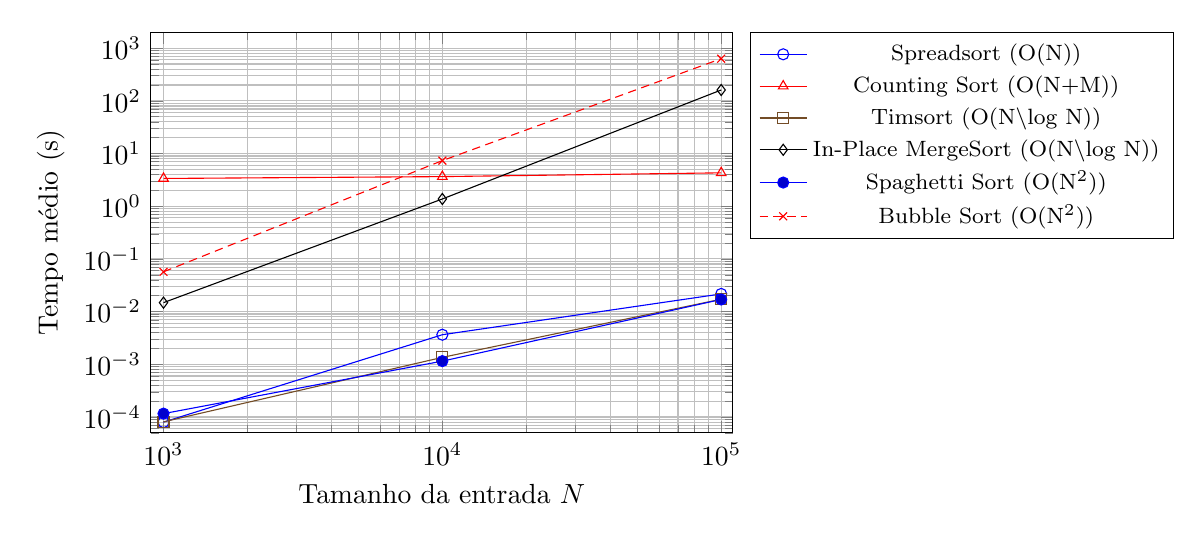
\begin{tikzpicture}
\begin{axis}[
    width=0.74\textwidth,
    height=0.55\textwidth,
    xmode=log,
    ymode=log,
    log basis x=10,
    log basis y=10,
    xlabel={Tamanho da entrada \(N\)},
    ylabel={Tempo médio (s)},
    % legend style={at={(0.02,0.02)},anchor=south west,font=\scriptsize},
     legend pos=outer north east,
    grid=both,
    xmin=900, xmax=110000,
    ymin=5e-5, ymax=2e3
]
% Dados: N = 1000, 10000, 100000

% O(N): Spreadsort
\addplot+[mark=o] coordinates {
    (1000, 0.000080)
    (10000, 0.003647)
    (100000, 0.021677)
};
\addlegendentry{\footnotesize Spreadsort (O(N))}

% O(N): Counting Sort
\addplot+[mark=triangle] coordinates {
    (1000, 3.366923)
    (10000, 3.652079)
    (100000, 4.305130)
};
\addlegendentry{\footnotesize Counting Sort (O(N+M))}

% O(N log N): Timsort
\addplot+[mark=square] coordinates {
    (1000, 0.000081)
    (10000, 0.001355)
    (100000, 0.017197)
};
\addlegendentry{\footnotesize Timsort (O(N\textbackslash log N))}

% O(N log N): In-Place MergeSort
\addplot+[mark=diamond] coordinates {
    (1000, 0.014808)
    (10000, 1.374327)
    (100000, 160.801455)
};
\addlegendentry{\footnotesize In-Place MergeSort (O(N\textbackslash log N))}

% O(N^2): Spaghetti Sort
\addplot+[mark=*] coordinates {
    (1000, 0.000116)
    (10000, 0.001150)
    (100000, 0.017013)
};
\addlegendentry{\footnotesize Spaghetti Sort (O(N\textsuperscript{2}))}

% O(N^2): Bubble Sort
\addplot+[mark=x] coordinates {
    (1000, 0.056984)
    (10000, 7.345069)
    (100000, 631.495185)
};
\addlegendentry{\footnotesize Bubble Sort (O(N\textsuperscript{2}))}

\end{axis}
\end{tikzpicture}
\caption{Comparação geral entre algoritmos representativos das três classes em escala log--log.}
\label{fig:comparacao-geral-loglog}
\end{figure}

Na Figura~\ref{fig:comparacao-geral-loglog} observam-se as seguintes tendências:

\begin{itemize}
    \item \textbf{Hierarquia esperada em termos de inclinação}: as curvas de \textit{Spreadsort} e \textit{Counting Sort} (quando se ignora o efeito de \(M\)) são menos inclinadas que as de \textit{Timsort} e \textit{In-Place MergeSort}, que por sua vez são menos inclinadas que as de \textit{Bubble Sort}. Isso é compatível com as ordens \(O(N)\), \(O(N\log N)\) e \(O(N^2)\).
    \item \textbf{Impacto das constantes}: \textit{Spaghetti Sort} (quadrático) acompanha de perto \textit{Timsort} (logarítmico) em toda a faixa de \(N\), e ambos são mais rápidos que \textit{Counting Sort} para \(N \geq 1000\). Isso evidencia que, para os tamanhos de entrada considerados e para este conjunto de dados, as constantes e o modelo de implementação podem ser mais determinantes que a classe assintótica isoladamente.
    \item \textbf{Gargalos de memória e estrutura de dados}: \textit{Counting Sort} e \textit{In-Place MergeSort} ilustram gargalos distintos. O primeiro é penalizado pelo tamanho do intervalo \(M\), que exige estruturas auxiliares enormes, enquanto o segundo sofre com a complexidade da fusão in-place, resultando em tempos comparáveis ou piores que algoritmos quadráticos clássicos.
\end{itemize}

\subsection{Consistência, Desvios Padrão e Outliers}

A análise dos desvios padrão permite avaliar a estabilidade dos algoritmos:

\begin{itemize}
    \item \textbf{Algoritmos muito rápidos} (\textit{Spreadsort}, \textit{Burstsort}, \textit{Flashsort}, \textit{Postman Sort}, \textit{Timsort}, \textit{Smooth Sort}, \textit{Spaghetti Sort}) apresentam desvios padrão muito pequenos em relação ao tempo médio (tipicamente abaixo de \(10\%\) e frequentemente abaixo de \(5\%\)), o que indica comportamento altamente determinístico e pouco sensível a variações do ambiente.
    \item \textbf{Algoritmos com grandes estruturas auxiliares} (\textit{Counting Sort}, \textit{Pigeonhole Sort}, \textit{Bucket Sort Integer}, \textit{In-Place MergeSort}, \textit{Tournament Sort}, \textit{Bubble Sort}, \textit{Gnome Sort}) exibem desvios padrão mais elevados, especialmente para grandes \(N\). Exemplos extremos incluem \textit{In-Place MergeSort} em \(N=100000\) (\(\text{DP} = 32{,}884374\) s) e \textit{Tournament Sort} em \(N=50000\) (\(\text{DP} = 1{,}143221\) s), sugerindo que o custo é fortemente afetado por detalhes de alocação, cache e possíveis interferências do sistema operacional.
\end{itemize}

Não foram observados valores isolados que destoassem completamente das tendências gerais; os tempos médios crescem de forma monotônica com \(N\) para todos os algoritmos, e os desvios padrão, embora altos em alguns casos, permanecem proporcionais aos tempos médios, o que indica ausência de outliers extremos nas 10 repetições.

\subsection{Síntese das Tendências Observadas}

Com base exclusivamente nos dados experimentais:

\begin{itemize}
    \item Algoritmos lineares independentes de \(M\) (\textit{Spreadsort}, \textit{Burstsort}, \textit{Flashsort}, \textit{Postman Sort}) e algoritmos \(O(N\log N)\) bem otimizados (\textit{Timsort}, \textit{Smooth Sort}, \textit{Merge Sort}, \textit{Quicksort}) apresentam os melhores tempos absolutos para todas as instâncias testadas.
    \item Algoritmos lineares dependentes de \(M\) (\textit{Counting Sort}, \textit{Pigeonhole Sort}, \textit{Bucket Sort Integer}) tornam-se impraticáveis neste conjunto de dados devido ao intervalo de valores (\(M \approx 3\times 10^7\)), superando em tempo até mesmo algoritmos \(O(N\log N)\) e alguns \(O(N^2)\) otimizados.
    \item Entre os algoritmos quadráticos, \textit{Shell Sort}, \textit{Comb Sort}, \textit{Recombinant Sort}, \textit{Strand Sort}, \textit{Spaghetti Sort}, \textit{Sorting Network} e \textit{Bitonic Sorter} destacam-se por tempos significativamente menores que os quadráticos clássicos, chegando a competir com algoritmos \(O(N\log N)\) para \(N=100000\).
    \item A hierarquia assintótica \(O(N) \subseteq O(N\log N) \subseteq O(N^2)\) é confirmada em termos de inclinação das curvas em escala log--log, mas há sobreposição substancial em termos de tempos absolutos, especialmente entre algoritmos quadráticos otimizados e algoritmos \(O(N\log N)\) com alto overhead, bem como entre algoritmos lineares dominados por \(M\) e algoritmos \(O(N\log N)\) eficientes.
\end{itemize}

\subsection{Limitações e justificativas}

Nesta seção são detalhados os itens que sofreram ajustes em relação à proposta inicial, bem como as justificativas para tais modificações. Durante o desenvolvimento do projeto, algumas alterações de escopo tornaram-se necessárias, especialmente no item referente à experimentação computacional.

Inicialmente, pretendia-se investigar o desempenho dos algoritmos utilizando instâncias de maior porte disponibilizadas pelo banco de vetores adotado. Entretanto, uma rodada experimental preliminar evidenciou que, mesmo para algoritmos com tempo de execução linear, o custo computacional já era elevado. Dessa forma, estender os testes para algoritmos de ordem logarítmica ou quadrática mostrou-se inviável dentro do prazo disponível para elaboração do estudo. Por esse motivo, conforme descrito no capítulo de Experimentos Computacionais, optou-se pela seleção de subconjuntos de instâncias com tamanhos específicos, suficientes para ilustrar o comportamento relativo entre os algoritmos, mas compatíveis com o tempo de execução acessível.

Outro ajuste necessário foi a decisão de realizar a comparação empírica apenas com as implementações em linguagem Python. Embora o projeto conte com implementações em outras linguagens, a execução de testes completos para todas elas demandaria recursos computacionais e temporais adicionais. Considerando que o objetivo central da análise é comparar o comportamento assintótico dos algoritmos, e que esse comportamento tende a se manter independentemente da linguagem utilizada, optou-se por concentrar a experimentação em uma única linguagem, decisão considerada suficiente e adequada ao propósito do estudo.

Por fim, apesar de terem sido implementados os algoritmos classificados como “miscelâneos”, não foi possível incluí-los na análise computacional. Alguns desses algoritmos apresentam tempo de pior caso não limitado superiormente — como o \textit{BogoSort} — tornando sua execução inviável no período disponível. Assim, este tópico e os outros citados acima permanecem como oportunidade para trabalhos futuros.

\section{Conclusões}
A análise experimental apresentada ao longo deste trabalho permitiu compreender de maneira aprofundada o comportamento prático dos diferentes algoritmos de ordenação quando submetidos a um conjunto padronizado de instâncias. Embora a teoria da complexidade ofereça uma previsão geral sobre o desempenho esperado, os experimentos revelam nuances importantes que somente a avaliação empírica é capaz de demonstrar.

Inicialmente, observou-se que os algoritmos lineares que não dependem do intervalo dos valores — como FlashSort, SpreadSort e Burstsort — apresentam desempenho excepcionalmente eficiente, mantendo tempos de execução muito baixos mesmo para entradas de cem mil elementos. Esse comportamento confirma não apenas a linearidade teórica, mas também evidencia a eficácia prática dessas implementações. Por outro lado, algoritmos lineares cuja complexidade envolve o parâmetro adicional \(M\), como Counting Sort e Pigeonhole Sort, mostraram-se impraticáveis diante de um intervalo extremamente amplo de valores. Este fenômeno ressalta a importância de analisar não apenas a ordem assintótica, mas também as condições reais de uso, especialmente quando o desempenho depende de características específicas dos dados.

Nos algoritmos classificados como \(O(N \log N)\), verificou-se que a diferença entre implementações pode ser significativa. Timsort, por exemplo, destacou-se pela estabilidade e excelente desempenho, muito em função de sua estratégia híbrida e da capacidade de explorar trechos já ordenados. Em contraste, algoritmos como In-place MergeSort e Tournament Sort apresentaram overhead elevado, evidenciando que uma boa complexidade teórica não garante necessariamente bom desempenho prático quando os custos internos da implementação são altos. Assim, fica claro que, dentro da mesma classe assintótica, a escolha do algoritmo mais adequado depende diretamente do contexto e das características específicas da aplicação.

Os algoritmos quadráticos, como previsto, demonstraram limitações severas conforme o tamanho das entradas aumentava. Bubble Sort e Gnome Sort tornaram-se inviáveis para instâncias maiores, com tempos de execução crescendo de forma abrupta. No entanto, algoritmos como Shell Sort e Comb Sort apresentaram desempenho consideravelmente melhor, mostrando que estratégias de melhoria podem reduzir drasticamente o impacto prático da complexidade quadrática pura. Mesmo assim, sua utilização em cenários de grande escala deve ser evitada quando alternativas mais eficientes estão disponíveis.

De modo geral, os resultados experimentais confirmam a hierarquia esperada entre as classes de complexidade, mas também demonstram que a prática envolve fatores adicionais, como otimizações internas, overhead computacional, consumo de memória e organização dos dados. Essa constatação reforça a importância de complementar a análise teórica com experimentos empíricos, garantindo que o algoritmo selecionado seja não apenas assintoticamente eficiente, mas também adequado às condições reais de uso.

Por fim, este estudo abre caminho para investigações futuras. Avaliações específicas do impacto de \(M\) nos algoritmos lineares baseados em contagem, análises detalhadas do consumo de memória ou ainda estudos comparativos em linguagens compiladas podem oferecer insights adicionais sobre o comportamento desses algoritmos em diferentes cenários. Ademais, é possível explorar as limitações ciadas no capítulo anterior, para complementação dos resultados já obtidos. A combinação entre análise teórica e experimental mostra-se, portanto, fundamental para a compreensão completa do desempenho de algoritmos de ordenação.